\documentclass[12pt]{article}

\setlength{\parindent}{0pt}
\setlength{\parskip}{2mm}

\usepackage{geometry}
 \geometry{
 letterpaper, left=20mm, right=20mm,  top=20mm,
 }
\usepackage{graphicx}
\graphicspath{ {graphics/} }
\usepackage{amssymb}
\usepackage[labelfont=bf]{caption}
\usepackage{listings}
\lstdefinestyle{standard}{
    numbers=left,
    tabsize=2,
    captionpos=b,
    language=C
}
\lstset{style=standard}

% Remove the following 3 lines when no longer in draft form
\usepackage{draftwatermark}
\SetWatermarkText{DRAFT}
\SetWatermarkScale{5}

%%%%%%%%%%%%%%%%%%%%%%%%%%%%%%%%%%%%%%%%%%%%%%%%%
\title{Transmission Protocol --- iCRAB}
%%%%%%%%%%%%%%%%%%%%%%%%%%%%%%%%%%%%%%%%%%%%%%%%%

\author{
	Noah Strong
}

\date{\today\ -- v1.0-wip}

\begin{document}

\maketitle

%\tableofcontents{}

\section{Introduction} \label{introduction}

The Crab Tracker project aims to provide a simple, efficient, reliable, and
cost-effective method for tracking crabs underwater. There are no accepted
standards that we're aware of for achieving the results we hope to achieve,
and to base our work too heavily off the work of existing products would
violate the clauses in the licenses of those products that protect against
reverse engineering.
For these reasons and more, we must define our own technologies and protocols.
Central to the project is the protocol that will be used to relay information
from transmitters (attached to crabs) to the central receiver (affixed to a
water-going vessel, such as a kayak).
Documented herein is that protocol, as well as the motivations and requirements
for many of the decisions behind it.
As of this writing, {\bf the protocol is still subject to change.}
We may find shortcomings or other problems with the protocol during
the prototyping stage of the product, at which point adjustments will be made.
This document will be updated as needed to reflect these changes,
and should always be treated as the official documentation for the protocol.

One of the major requirements of this project is the ability for each
individual transmitter to be uniquely identifiable. Therefore, we must encode
the device's unique identifier (herein referred to as the ID or UID) in each
signal that the device broadcasts.
% TODO - add reference to appropriate section
We will discuss this in section $<\dots>$.%\ref{background}.

Additionally, because all transmitters transmit at the same audio frequency
(baseband signaling), it is possible for multiple transmitters to transmit
simultaneously. We want such collisions to be detectable by the receiver
so that invalid data is never presented to the user. Simple implementations
of an encoding protocol can lead to situations in which collisions are not
detectable, but the protocol proposed in this document aims to prevent the
possibility of undetectable collisions. For a further discussion on how
collisions may arise, proposed solutions, and other background information,
please see RFC 1.

\section{Background} \label{background}

For a thorough background on some of the challenges faced in designing this
protocol, please refer to the RFC-1 ``Collision Detection'' document.

To satisfy the requirements of this project, we are designing a new protocol.
This protocol will encode the UID of each transmitter in such a way that
collisions (multiple simultaneous transmissions by different transmitters) can
be detected by a receiving station and discarded.
The protocol is a simple
series of HIGH and LOW audio signals operating at a predefined
frequency. (The specific frequency to be used will be documented elsewhere
on the hardware engineering side of things.)
The series of ``pings'' and the separation between them will be organized in a
specific pattern based on the UID of the given transmitter, known as the
Unique Transmission Pattern (or UTP for short).

Additionally, we may want to have the ability to detect when a transmitter
has stopped moving, possibly because the crab molted its shell or died.
In this case, we want each broadcast to not only encode the UID of the
transmitter, but also some boolean value (such as $isInert$).
To this end, we introduce a potential second encoding for each signal that
will be used only if this boolean value is true.
While the boolean value could theoretically represent any piece of data about
the transmitter, we will assume herein that it refers to the $isInert$
variable.

We label this protocol the id-correlated rhythmic audio broadcast protocol,
or iCRAB for short.

\section{iCRAB Protocol Definition} \label{protocol-def}

\subsection{Overview}

%Occasionally, on a randomly varying interval, each transmitter will broadcast
%a single burst of information.
At the core of this protocol is a single bust of information which is
transmitted repeatedly on some randomly-varying interval.
This burst of data, transmitted via acoustic waves, will encode the unique
identifier of the given transmitter. The burst, hereafter referred to as a
unique transmission pattern (UTP), will consist of two pings (short, continuous
transmissions of the carrier frequency), separated by some delay time $d$.
The duration of the pings and the delay time $d$ will be functions of the
transmitter's UID.
The interval between UTPs will be random, and each transmitter will recalculate
the interval time after each UTP according to a shared formula.
See Figure \ref{fig:utp} for an example of a UTP.

\begin{figure}[h]
\centering
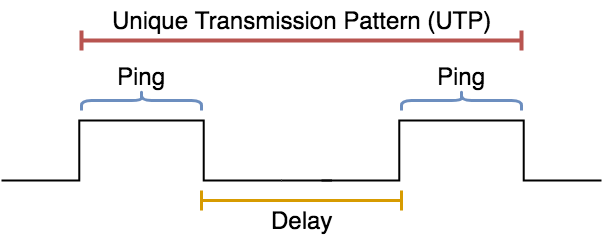
\includegraphics[scale=0.5]{utp}

\caption{A Unique Transmission Pattern}\label{fig:utp}
\end{figure}

In general, he duration of the two pings will be identical.
However, this may change depending on how we encode an additional boolean
value in the signal.
See RFC 2 for more details.

\subsection{Rationale and Related Information} \label{rationale}

Based on John's rough estimate early in the project, we will initially
comply with the following constraints.

\begin{enumerate} \itemsep -2pt
	\item The minimum ping duration should be 1 millisecond.
	\item The ``step size'' (i.e. smallest difference in duration between
		any two pings) should be 0.1 milliseconds.
	\item The minimum delay duration should be 10 milliseconds.
	\item The ``step size'' for the delay should also be 0.1 milliseconds.
\end{enumerate}

Additionally, we expect that transmitting every 30 seconds should provide
the user with frequent enough location updates to be practical, but that
transmissions will also be
infrequent enough that the expected number of collisions is very low.
For more information on collision statistics, see the document titled
{\em RFC1\_stats.pdf}.

Observe, however, that if every transmitter transmitted on a fixed interval,
then we could theoretically encounter a situation in which two transmitters
transmit at almost exactly the same time for the entire duration of their
deployment.
In other words, their transmissions would always collide, and the receiver
would never be able to reliably determine the location of either one.
To remedy this, we will instead randomly vary the interval between broadcasts.
That way, if two transmitters happen to transmit at the same time,
they won't necessarily collide the second time around.
The random adjustment will need to be recalculated for each interval in order
to reduce our chances of collisions.

Finally, this protocol will be capable of uniquely encoding up to 500*
identifiers.
Each ID will be a number in the range $[0, MAX\_UID)$.

* Note: this number may change based on the boolean encoding method we choose
to use. See RFC 2.

\subsection{Preamble to Definitions and Specifications} \label{preamble}

Each Unique Transmission Pattern (UTP) will be formed by a ping, a delay,
and another ping, in that order.
Each transmitter will broadcast a UTP and will then wait for some interval
before transmitting a UTP again.
This process loops infinitely throughout the transmitter's lifetime.

Defined in Table \ref{table:constants}) are the constants that we will use for
the various aspects of this protocol.
This section of the document will be updated as needed if these values
change.

Table \ref{table:formulae} lists the various mathematical formulae we will
use for encoding.
Some functions are passed a single integer value, which is a UID.

Finally, we formally define the behavior of a transmitter in pseudo-code
(see Listing \ref{lst:tx}.)
The functions {\em HIGH} and {\em LOW} cause the physical transmitter to begin
or cease transmitting, respectively.
The {\em sleep()} function simply causes execution of teh code to stop for a
given number of milliseconds.

\newpage
\subsection{iCRAB Definitions and Specifications} \label{specs}

This section aims to be the developer's one-stop shop for relevant constants,
formulae, and other definitions.

\begin{table}[ht]
\centering
\begin{tabular}{|l|l|}
\hline
Variable & Value \\
\hline
MIN\_INTERVAL	&	25 ms	\\
MAX\_INTERVAL	&	35 ms	\\
MAX\_ID			&	499		\\
MIN\_PING\_DUR	&	1.0 ms	\\
MIN\_DELAY\_DUR	&	10.0 ms	\\
STEP\_SIZE		&	0.1	ms	\\
\hline
\end{tabular}
\caption{Constants to be used for the iCRAB Protocol}\label{table:constants}
\end{table}

\begin{table}[ht]
\centering
\begin{tabular}{|c|l|}
\hline
Function Name & Expression \\
\hline
ping(id)		&	$(id \times STEP\_SIZE)+MIN\_PING\_DUR$	\\
delay(id)	&	$(id \times STEP\_SIZE)+MIN\_DELAY\_DUR$	\\
interval()	&	$randInRange(MIN\_INTERVAL, MAX\_INTERVAL)$	\\
\hline
\end{tabular}
\caption{Formulae to be used for the iCRAB Protocol}\label{table:formulae}
\end{table}


\begin{lstlisting}[caption={Transmitter Behavior},label={lst:tx}]
void doPing(int id){
	HIGH()
	sleep(ping(id))
	LOW()
}

void loop(id){
	doPing(id)
	sleep(delay(id))
	doPing(id)
	sleep(interval())
}
\end{lstlisting}

\begin{figure}[h]
\centering
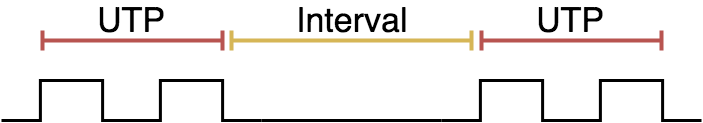
\includegraphics[scale=0.5]{interval}

\caption{For reference, pictured are two UTPs separated by an interval}
\label{fig:interval}
\end{figure}

%%%%%%%%%%%%%%%%%%%%%%%%%%%%%%%%%%%%%%%%%%%%%%%%%%%%%%%%%%%%%%%%%%%%%%%%%%%%%%%
% APPENDIX
%%%%%%%%%%%%%%%%%%%%%%%%%%%%%%%%%%%%%%%%%%%%%%%%%%%%%%%%%%%%%%%%%%%%%%%%%%%%%%%

\newpage
\appendix
\section{Glossary of Terms} \label{glossary}

{\bf Delay:}
	in the context of ID encoding, the space between the falling edge of one
	{\bf ping} and the rising of the next within a single {\bf UTP}.

{\bf Delay Time ({\em d}):}
	the duration (generally in milliseconds) of a given {\bf delay}.

{\bf iCRAB (id-correlated rhythmic audio broadcast) protocol:}
	the protocol designed by the members of the Crab Tracker project and
	described in detail in this document.

{\bf Inert:}
	A transmitter will be marked as {\bf inert} if it is determined that the
	transmitter has not moved ``enough'' in a given period of time.
	This definition is subject to changes and hardware constraints, and
	refers to an experimental addition to the project's requirements that
	has yet to be implemented or fully defined in writing.

{\bf Interval:}
	the time between two consecutive broadcasts of {\bf UTP}. Measured by the
	distance between the final falling edge of one ping and the first rising
	edge of the next.

{\bf Ping:}
	a single, continuous transmission of signal.

{\bf Ping Duration:}
	the length of time between the rising and falling edges of a continuous
	transmission (a {\bf ping}).

{\bf Unique Transmission Pattern, UTP:}
	a sequence of two {\bf ping}s separated by some {\bf delay} used to
	encode the unique identifier of a transmitter.

\end{document}

